% GitHub's PDF preview requires classic cross-reference tables; PDF 1.5
% object streams render as "invalid PDF" there.
\pdfminorversion=4
\pdfobjcompresslevel=0
\documentclass[11pt,a4paper]{article}

\usepackage[margin=2.6cm]{geometry}
\usepackage{amsmath}
\usepackage{booktabs}
\usepackage{graphicx}
\usepackage{microtype}
\usepackage{natbib}
\usepackage[hidelinks]{hyperref}
\usepackage{caption}
\captionsetup{font=small,labelfont=bf}

\title{Momentum and Profitability in European Small-Cap
Equities\thanks{Research
summary of a private codebase (data pipeline, backtest engine, test suite,
and research log). Source code and the full chronological research record
are available on request. This document describes research output only and
is not investment advice.}}
\author{Johannes Benthaus\\
  \small\texttt{johannes.benthaus@gmail.com}}
\date{July 2026}

\begin{document}
\maketitle

\begin{abstract}
\noindent
This document summarizes the construction and evaluation of a cross-sectional
equity strategy on European small caps (EUR 180M--1.8B market capitalization,
15 markets, 2007--2025), built on point-in-time Compustat Global data. A
two-factor composite of 12--2 momentum and gross profitability
\citep[cf.][]{jegadeesh1993,novymarx2013}, held long-only in the top decile
with monthly rebalancing, earns an annualized excess return of 9.7\% over the
equal-weighted universe out of sample (2020--2025; Newey--West $t = 4.41$,
information ratio 1.42), against 9.8\% ($t = 5.83$) in sample. A variant
replacing annual gross profitability with quarterly income-before-extraordinary-items
over assets earns 15.4\% ($t = 4.54$) out of sample. A market-neutral
implementation, shorting a European small-cap ETF against the long book with a
rolling 24-month hedge ratio, attains an out-of-sample net Sharpe ratio of
1.4--1.7 for the quarterly variant, with CAPM market beta statistically
indistinguishable from zero. A capacity study replays the strategy under
participation-limited execution and puts the useful ceiling near EUR 500M.
Data-integrity safeguards, cost sensitivity, and methodological limitations
are documented, including partial reuse of the holdout window across research
iterations.
\end{abstract}

\section{Overview}

The project implements a monthly cross-sectional factor model for European
small-cap equities: universe construction from point-in-time vendor data,
factor computation under explicit publication-lag assumptions, a long-only
decile backtest with an in-sample/out-of-sample split fixed in advance, and
post-hoc diagnostics (factor-model alphas, country attribution, tail
behavior). Two further sections address implementation: a market-neutral
overlay that shorts a European small-cap ETF against the long book, and a
capacity study that replays the strategy under an explicit execution model
with daily participation limits. The emphasis throughout is on the mechanics
that make backtest numbers trustworthy: look-ahead prevention,
data-integrity checks, and test-enforced invariants. The factor signals
themselves are deliberately taken from the published literature.

\section{Data and universe}
\label{sec:data}

\paragraph{Sources.} Security-level daily prices, shares outstanding, and
listing metadata are from Compustat Global via WRDS. Annual and quarterly
fundamentals come from \texttt{g\_funda} and \texttt{g\_fundq}.
Foreign-exchange conversion uses ECB daily reference rates, and all returns
are converted to EUR at month-end rates.

\paragraph{Universe.} At each month-end formation date the universe comprises
firms (i) legally incorporated in one of 15 European countries,\footnote{GBR,
DEU, FRA, NLD, SWE, CHE, ITA, ESP, BEL, DNK, NOR, FIN, AUT, IRL, PRT.
Incorporation proxies operating exposure; the mismatch (holding companies,
domiciled multinationals) is predominantly a large-cap phenomenon and is
small in this size segment.} (ii) with a European primary ordinary listing, and
(iii) with company-level market capitalization, aggregated across listings
and share classes, between EUR 180M and EUR 1{,}800M. Financial-format
filers (banks, insurers) are excluded via the industrial-format
(\texttt{INDL}) filter on fundamentals. The filtered universe averages 927
names per month in sample and 1{,}024 out of sample.

\paragraph{Returns.} Monthly returns are computed from daily closes at the
level of the individual security line, with a data-error filter that removes
monthly returns outside $[-90\%, +200\%]$. Returns are price-only: the vendor's
total-return adjustment is not of usable quality in this segment, so both
strategy and benchmark returns exclude dividends
(Section~\ref{sec:limitations}).

\section{Factors and timing discipline}
\label{sec:factors}

Two production strategies are evaluated, both equal-weighted composites of
two cross-sectional percentile ranks:

\begin{itemize}
  \item \textbf{MP} (research reference): 12--2 momentum
  \citep{jegadeesh1993,carhart1997} plus gross profitability, $(\mathrm{REVT}
  - \mathrm{COGS})/\mathrm{AT}$, from annual filings \citep{novymarx2013}.
  \item \textbf{MI} (implementation variant): 12--2 momentum plus quarterly
  profitability, income before extraordinary items over total assets
  ($\mathrm{IBQ}/\mathrm{ATQ}$), a quarterly ROA-family measure in the spirit
  of the $q$-factor profitability literature \citep{hou2015}. Its rationale
  is signal freshness: the quarterly measure updates four times a year, the
  annual one once. The choice between MP and MI was, however, made with
  out-of-sample results visible (Section~\ref{sec:limitations}).
\end{itemize}

Accruals \citep{sloan1996} and asset growth \citep{cooper2008} were also
evaluated. Both carry significant Fama--MacBeth coefficients, but their
composites underperform the profitability variants in the decile backtest and
were not selected.

Timing rules are uniform. Accounting data enters factor ranks only from
filing availability, proxied as fiscal period end plus 90 days
because Compustat Global provides no report dates, and filings drop out of
the ranks after a staleness cap. The merge is a backward as-of join, so no
filing can enter a formation month before its availability date. Momentum and forward returns use exact
calendar-month lookups that treat listing gaps as missing observations.
Portfolio selection never conditions on forward
return availability. These invariants are enforced by runtime assertions and
a test suite (Section~\ref{sec:software}).

\section{Backtest design}
\label{sec:backtest}

At each formation month-end, stocks are ranked on the composite, and the
top decile of roughly 100 names (D10) is held equal-weighted for one
month. The benchmark is the equal-weighted factor-eligible universe, which
removes the small-cap and universe-construction tilts from the excess return.
The in-sample period covers formations 2007--2019 (156 months) and the
out-of-sample period 2020--2025 (71 months). The split date was fixed before
evaluation and never moved. Significance of mean monthly excess returns uses Newey--West standard
errors with 12 lags. Sharpe ratios are computed with a zero risk-free rate
and are therefore overstated by roughly $r_f/\sigma$ for long-only series,
about 0.09 over this out-of-sample window. Excess returns, their
$t$-statistics, and information ratios are unaffected. Transaction costs are
charged at 30\,bps round-trip against realized turnover
(Section~\ref{sec:results}).

\section{Long-only results}
\label{sec:results}

Table~\ref{tab:headline} reports the headline results.
Figures~\ref{fig:cumulative} and~\ref{fig:deciles} show the cumulative path
and the out-of-sample decile ladder for MP.

\begin{table}[t]
\centering
\small
\begin{tabular}{llrrrrrr}
\toprule
Strategy & Period & Excess & $t$ & Sharpe & IR & Max DD & Turnover \\
\midrule
MP & IS  (2007--19) & +9.8\%  & 5.83 & 0.97 & 1.49 & $-52\%$ & 265\% \\
MP & OOS (2020--25) & +9.7\%  & 4.41 & 0.75 & 1.42 & $-25\%$ & 261\% \\
MI & IS  (2007--19) & +13.5\% & 6.67 & 1.16 & 1.92 & $-53\%$ & 314\% \\
MI & OOS (2020--25) & +15.4\% & 4.54 & 1.04 & 2.03 & $-25\%$ & 314\% \\
\bottomrule
\end{tabular}
\caption{D10 long-only performance, EUR, price-only returns, gross of costs.
Excess is the annualized mean monthly return over the equal-weighted
universe; $t$ uses Newey--West standard errors (12 lags); IR is the
information ratio versus the same benchmark; turnover is annualized one-sided
turnover. Sharpe ratios use a zero risk-free rate
(Section~\ref{sec:backtest}). At the 30\,bps round-trip cost assumption the
annual drag is 0.78\% (MP) and 0.94\% (MI); the break-even round-trip cost
that zeroes out-of-sample excess is $\approx$370\,bps (MP) and
$\approx$490\,bps (MI).}
\label{tab:headline}
\end{table}

Three observations. First, out-of-sample decay relative to in-sample is
minimal for MP (9.8\% $\to$ 9.7\%) and absent for MI, though
Section~\ref{sec:limitations} qualifies how much weight the out-of-sample
figures can bear. Second, the decile ladder (Figure~\ref{fig:deciles}) is
approximately monotone with a strongly negative bottom decile, consistent
with a genuine cross-sectional signal rather than a handful of outliers.
Third, the benchmark-relative construction makes the excess robust to the
segment's overall performance: the equal-weighted universe returned only
2.6\% annualized out of sample.

\paragraph{Factor-model alphas.} MP D10 long-only returns, converted to USD
to match the factor basis, are regressed out of sample on the European
Fama--French factors \citep{fama2015} plus momentum, with Newey--West
(4 lags) standard errors. This gives CAPM $\alpha = +4.1\%$ ($t{=}0.88$),
FF3 $\alpha = +9.2\%$ ($t{=}3.18$), and FF6 $\alpha = +3.0\%$ ($t{=}1.23$),
with loadings concentrated where the construction puts them: SMB $+1.19$
and UMD $+0.44$, both $p<0.01$. The strategy's return is thus largely compensation
through known factor channels deliberately loaded:
the FF6 alpha is statistically indistinguishable from zero once a
broad-market momentum factor is allowed to absorb the momentum sleeve. What the long-only premium adds
over passive factor exposure is decile concentration: a top-decile sort on
small caps, against the factor's 30\%-breakpoint construction on all
caps.

\begin{figure}[t]
\centering
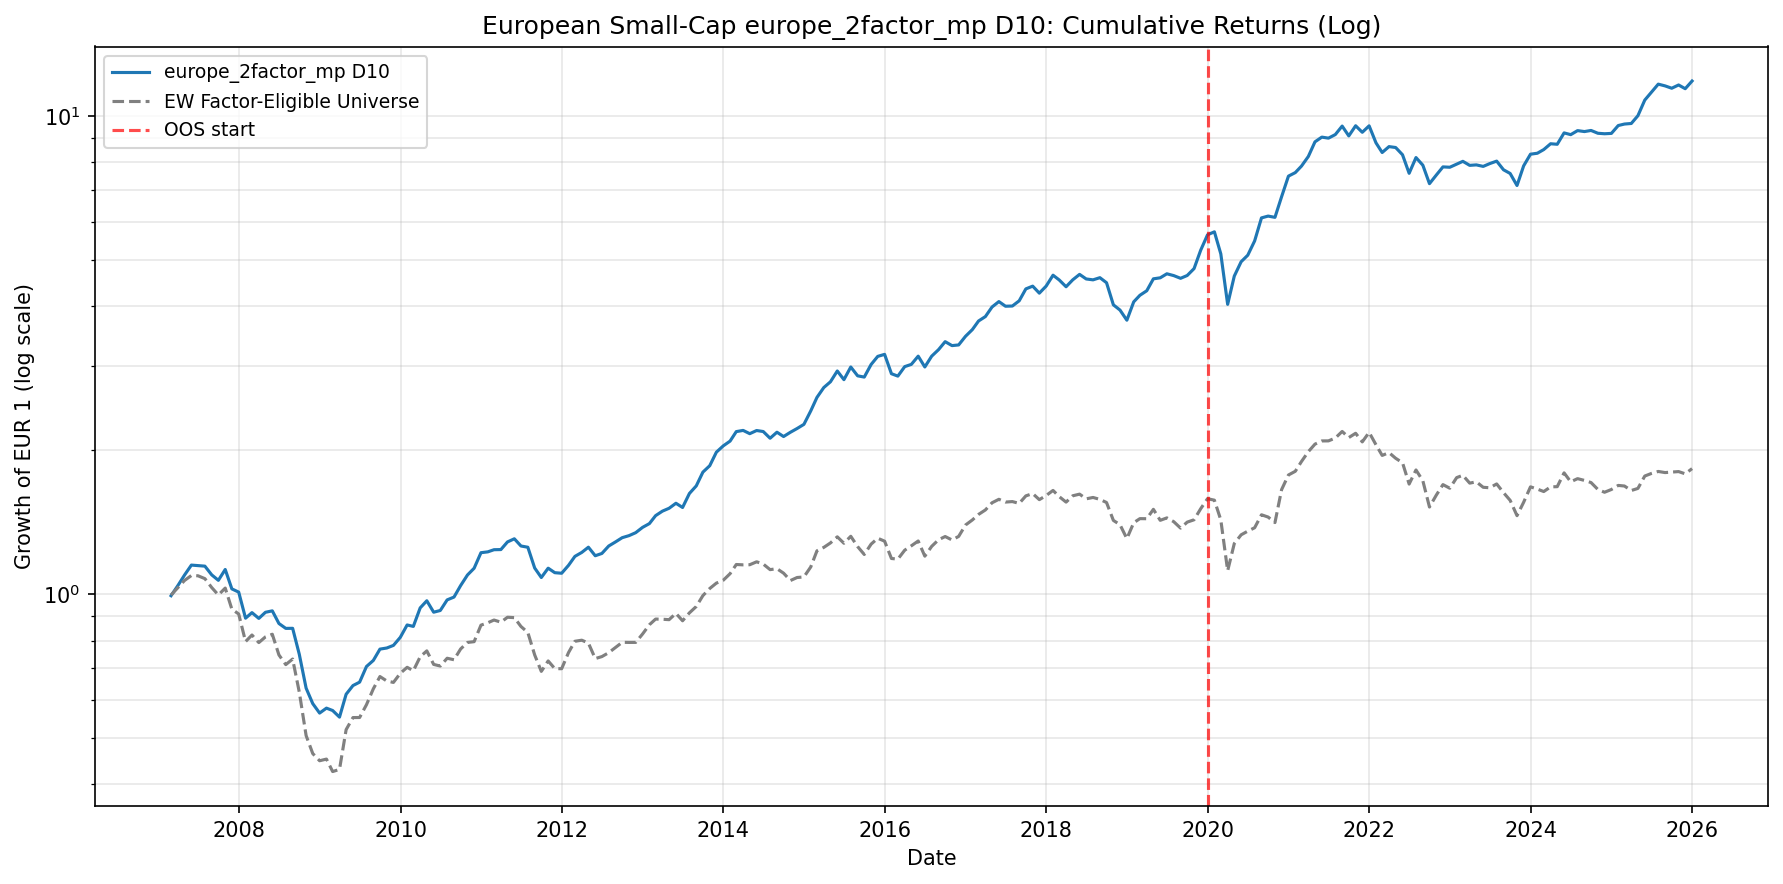
\includegraphics[width=\textwidth]{europe_backtest_cumulative_log.png}
\caption{Cumulative growth of EUR 1 (log scale), MP D10 versus the
equal-weighted factor-eligible universe, price-only returns, gross of costs.
The vertical dashed line marks the out-of-sample split (2020-01), fixed
before evaluation.}
\label{fig:cumulative}
\end{figure}

\begin{figure}[t]
\centering
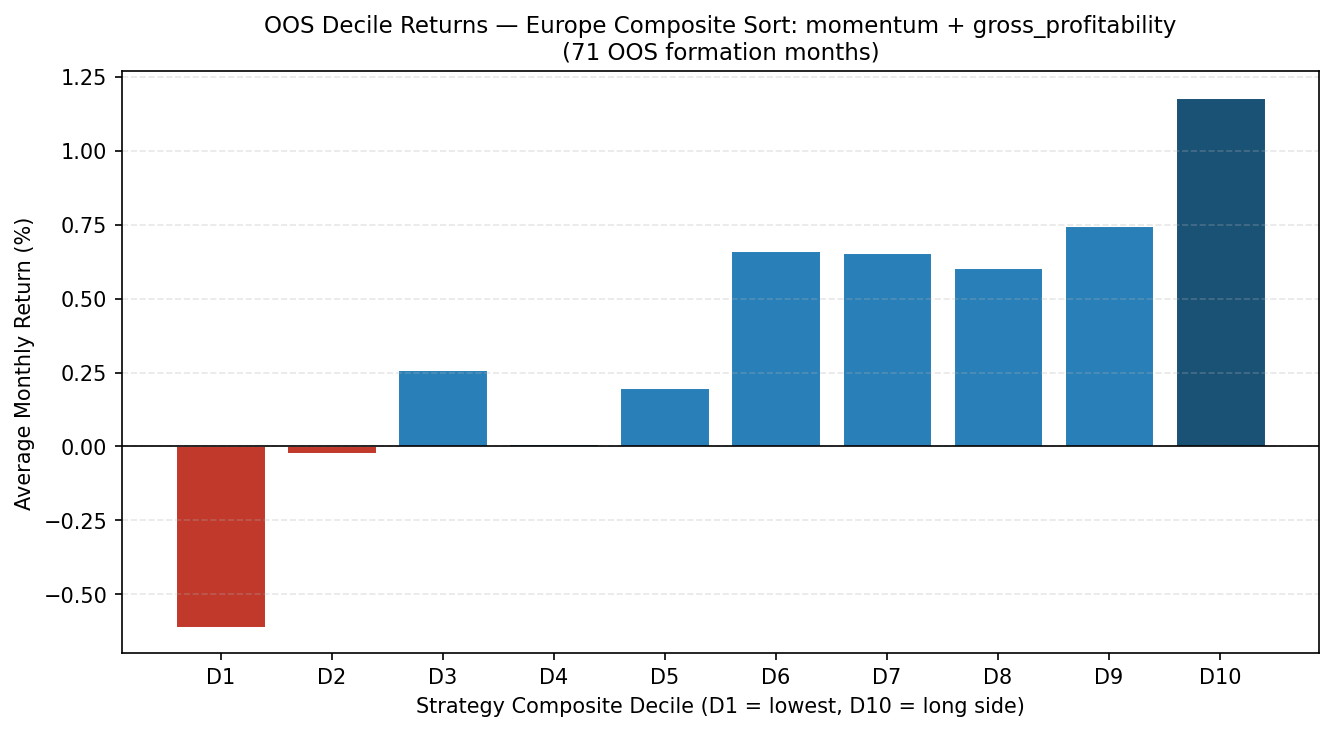
\includegraphics[width=0.85\textwidth]{oos_decile_spread.png}
\caption{Average monthly return by composite decile, MP, out-of-sample
(71 formation months). D10 is the long side of the production strategy.}
\label{fig:deciles}
\end{figure}

\section{Market-neutral implementation}
\label{sec:hedged}

A tradable market-neutral variant shorts XXSC.DE (Xtrackers MSCI Europe
Small Cap UCITS ETF, accumulating share class) against the D10 book. The
hedge ratio is a trailing 24-month OLS beta re-estimated monthly on months
$[T{-}24, T{-}1]$, so no information from the hedged month enters its own
hedge ratio. A 50\,bps annual borrow cost is charged on the short leg. The
long side is price-only while the accumulating ETF's price series is
total-return, so results are bracketed by a flat dividend adjustment on the
long side of $[0\%, +2\%]$ per year. The lower bound is assumption-free and
understates by the long book's actual dividend yield. The upper bound is a
conservative estimate of the segment's yield.

\begin{table}[t]
\centering
\small
\begin{tabular}{lrrrr}
\toprule
 & \multicolumn{2}{c}{Net of all modeled costs} & \multicolumn{2}{c}{CAPM (gross of trading cost)} \\
\cmidrule(lr){2-3}\cmidrule(lr){4-5}
Strategy & Ann.\ return & Sharpe & $\beta_{\mathrm{Mkt}}$ ($t$) & $\alpha$ ($t$) \\
\midrule
MI hedged & +12.3\% -- +14.3\% & 1.44 -- 1.68 & $-0.03$ ($-0.6$) & +13.5\% -- +15.5\% (3.0--3.4) \\
MP hedged & +6.2\% -- +8.2\%   & 0.85 -- 1.13 & $-0.02$ ($-0.4$) & +7.2\% -- +9.2\% (2.2--2.8) \\
\bottomrule
\end{tabular}
\caption{Hedged D10, out-of-sample (71 months). Newey--West $t$-statistics in
parentheses; for the $\alpha$ column the two $t$-values correspond to the two
ends of the reported range. Ranges span the $[0\%, +2\%]$
dividend adjustment; the hedge ratio is invariant to it. ``Net'' deducts the
50\,bps borrow and long-side trading cost at 30\,bps~$\times$~turnover.
Volatility is 8.5\% (MI) and 7.3\% (MP) throughout. Sharpe ratios use a zero
risk-free rate; the spread is self-funding, so this coincides with the
standard excess-return definition. Regressions use
Newey--West (4 lags) on the EUR spread.}
\label{tab:hedged}
\end{table}

Market neutrality is read off the unconditional CAPM beta, which is
statistically zero for both strategies out of sample
(Table~\ref{tab:hedged}). The residual beta against the hedge instrument
itself is likewise zero ($-0.03$, $t{=}-0.55$). Neutrality is not factor
neutrality: the hedged book intentionally retains small-cap and momentum
exposure, with FF6 loadings of SMB $\approx +0.5$ and UMD
$\approx +0.33$--$0.42$, both significant. Its FF6 alpha out of sample is
$+12.8\%$--$+14.8\%$ ($t \geq 3.5$) for MI but only $+4.4\%$--$+6.4\%$
($t = 1.7$--$2.5$) for MP, so factor-adjusted-alpha claims rest on MI.

The factor returns are USD-based. A funded portfolio carries the EURUSD
move at first order, so the long-only returns of Section~\ref{sec:results}
are converted to USD before regression. The zero-notional spread has no
principal to translate: its EUR and USD measurements differ only by a
second-order cross term, and it is regressed in EUR. Converting the
collateral as well would add its full EURUSD return.

\section{Capacity}
\label{sec:capacity}

A separate capacity study replays the strategy under an explicit execution
model:

\begin{itemize}
  \item \emph{Participation limits.} A position in name $i$ is built or
  unwound at up to a daily participation rate $p$ of the name's daily
  traded euro volume $V_i$, for at most $d$ trading days per rebalance.
  The per-name weight cap is therefore
  \[
    c_i \;=\; \frac{d \cdot p \cdot V_i}{\mathrm{AUM}}.
  \]
  The budget $d \cdot p$ per unit of AUM determines which books are
  feasible. Halving the participation rate roughly halves each AUM tier.
  \item \emph{Conservative volume measurement.} The volume $V_i$ entering
  the caps is the trailing 63-day median of euro volume on the
  primary listing. Small-cap volume is right-skewed, with a mean around 1.4 times
  the median, so a mean-based measure admits names on the strength of
  single block-print days. The median basis is roughly 30\% tighter.
  Volume on secondary venues is ignored, which understates consolidated
  liquidity by roughly 13\% overall. The names that hit their caps are
  predominantly single-listed, however, so this moves results by at most
  about 0.1 points per cell.
  \item \emph{Liquidity floor.} Names are excluded before selection
  unless they traded on at least 50 of the trailing 63 days, with a mean
  daily volume of at least EUR 100k and at least 0.05\% of market
  capitalization. The thresholds were fixed upfront on
  execution-feasibility grounds. The floor removes about 27\% of
  top-decile names, the same share it removes from the full universe, and
  leaves the excess return unchanged, direct evidence that the edge does
  not depend on the least liquid names.
  \item \emph{Allocation.} Where caps bind, the book is market-cap-weighted
  within per-name caps, and capital a capped name cannot absorb spills to
  the next names in factor-rank order.
  \item \emph{Costs and scope.} All trades pay the 30\,bps round-trip
  cost, including forced sales. These arise when a held name drops out of
  the universe, mostly by appreciating past the market-cap ceiling, or
  when a position comes to exceed what its diminished volume could
  liquidate within the exit window. The simulation books these exits at
  month-end prices. That flatters ceiling exits, because the price move
  that causes the exit also sets the sale price, and penalizes
  volume-collapse trims, because the median understates the volume
  actually available in those names. Together the two effects move
  results by at most about 0.3 percentage points annualized. Price impact
  of the trading itself is not modeled: the participation cap is the
  model's only impact control, and every figure is pre-slippage.
\end{itemize}

Two findings organize the results. First, the signal decays slowly in the
holding horizon: pre-cost, a quarterly rebalance retains roughly 87\% of the
monthly alpha, and a semi-annual one about 70\%. The effective lever at
scale is therefore the execution budget rather than the rebalance label. Second, the binding
constraint is structural rather than per-name illiquidity: alpha concentrates
at the smaller end of the 180--1{,}800M band, so capacity-driven reallocation
pushes the book toward larger names where the factor edge is weakest.

Configurations with equal execution budgets admit the same portfolio, but a
longer build window at a lower participation rate places a smaller daily
footprint in the market for the same book. The recommended operating mode
therefore spends the budget as monthly rebalancing with a 120-trading-day
build window at 3\% daily participation and a 60-trading-day exit ceiling
at 10\%. Operationally, a name's per-rebalance entry trade is capped at
what 3\% of its median daily volume executes in 120 trading days, or
$d \cdot p = 3.6$ days of volume. Because that window is several times the month between
rebalances, a large position is worked continuously across successive
rebalances toward its moving target. The exit ceiling caps the held
position itself at what 10\% of median daily volume liquidates in 60
trading days, or 6 days of volume, so a position at the ceiling clears in
about three monthly rebalances. Names that leave the selection are unwound
under the same rate limits. Median positions sit at 3--15\% of the exit
ceiling. The mode is the best-performing configuration on the tested grid
of 90- and 120-day build windows and 30- to 60-day exit ceilings.
Configurations outside this grid were not tested.

Table~\ref{tab:capacity} reports the mode's net excess by AUM tier. The
useful ceiling is near \textbf{EUR 500M}. A quarterly alternative, a
30-day build window at 10\% participation with no ceiling on held
positions, prints higher paper alpha at the largest tier: MP $+6.0\%$ and
MI $+8.1\%$ at EUR 500M. It buys that by trading at more than three times
the daily participation, and it holds 41--46\% of NAV above what one
month's volume could liquidate, against 14--17\% under the recommended
mode. A flat 5\% NAV position cap, added for single-name concentration
control, costs within measurement noise at every tier except MP at EUR
500M. There it costs about 1.1 points full period and 2.5 out of sample,
so a looser cap is indicated.

A square-root argument puts a scale on the unmodeled price impact.
Empirically, the cost per euro of a worked order follows
\[
  \text{cost per euro} \;\approx\; Y \cdot \sigma \cdot \sqrt{\frac{Q}{V}},
\]
with $Y \approx 0.5$, $\sigma$ the daily volatility, and $Q/V$ the order's
total size in days of volume \citep{toth2011}.
Applied to a build spread over months, the law brackets the cost, because
the impact of earlier trading partially decays while the order is still
being worked \citep{bouchaud2004}. If impact
decayed fully between daily slices, every euro traded at 3\% participation
would pay roughly 15--20\,bps one-way at $\sigma \approx 2\%$. If the full
build carried its impact to completion, a build at the cap of 3.6 days of
volume would pay about 2\%, and the median position of 0.2--0.9 days of
volume 40--100\,bps. Combined with the mode's roughly 250\% annual
turnover, the implied drag at EUR 500M is on the order of 0.4 percentage
points annualized under fast decay and 1--2 under full memory, with builds
worked over weeks to months falling between. The regimes also scale
differently: under fast decay the drag is set by the participation rate
and is nearly flat across AUM tiers, while under full memory it grows
roughly as $\sqrt{\mathrm{AUM}}$, steepening the gradient of
Table~\ref{tab:capacity}. This is an order-of-magnitude illustration only.
Even at the full-memory end, MI retains a clear margin at EUR 500M, while
the MP margin there becomes thin.

\begin{table}[t]
\centering
\small
\begin{tabular}{llrr}
\toprule
AUM & Execution & MP & MI \\
\midrule
$\leq$ EUR 15M & monthly, equal-weighted & +8.2\% & +11.2\% \\
EUR 100M & monthly, 120-day build at 3\% & +6.1\% & +9.8\% \\
EUR 250M & monthly, 120-day build at 3\% & +5.4\% & +8.0\% \\
EUR 500M & monthly, 120-day build at 3\% & +4.4\% & +7.4\% \\
\bottomrule
\end{tabular}
\caption{Annualized net excess return (full period) by AUM tier under the
capacity simulation, each tier at its recommended operating mode. The
simulation's execution conventions differ from the production backtest of
Table~\ref{tab:headline}, so levels are indicative and the gradient across
AUM tiers is the result.}
\label{tab:capacity}
\end{table}

\section{Robustness and limitations}
\label{sec:limitations}

\begin{enumerate}
  \item \textbf{Reuse of the holdout window.} The 2020-01 split was fixed
  before evaluation and never moved, and selection never conditions on
  forward returns. The out-of-sample window was, however, evaluated
  repeatedly across research iterations: strategy variants were compared
  on out-of-sample statistics, and the out-of-sample impact of data
  corrections was monitored. Repeated exposure to a fixed holdout is implicit
  selection. The reported out-of-sample figures are not a one-shot test, and
  the size of the resulting upward bias cannot be estimated from within the
  sample. Three things mitigate. The factor set is small and taken from
  prior literature rather than mined from this data. Data corrections were
  accepted on correctness and moved results in both directions. And the
  headline $t$-statistics ($\geq$4.4) survive substantial haircuts. The
  natural unbiased test is prospective evaluation on data realized after
  this research.
  \item \textbf{Price-only returns.} Absolute returns are understated by
  approximately the segment's dividend yield, estimated at around 2\% per
  year. Excess returns versus the equal-weighted universe are approximately
  unaffected, since both sides omit dividends. The hedged results bracket
  the resulting asymmetry explicitly.
  \item \textbf{No delisting returns.} Compustat Global provides none, so
  exits enter as missing forward returns. A stress test classifying all
  1{,}179 permanent exits via vendor deletion-reason codes finds 60\% coded
  as M\&A against 1.3\% as failures, with exits concentrated in the top
  decile. The missing returns are therefore more likely to be positive
  acquisition premia than losses. Imposing
  $-100\%$ on every exit still leaves out-of-sample excess positive
  ($+5.0\%$, $t{=}1.70$, evaluated at an earlier pipeline vintage).
  \item \textbf{Transaction costs are an assumption.} 30\,bps round-trip is
  anchored to quoted European small-cap spreads (15--60\,bps) and the
  academic cost literature \citep{frazzini2015,novymarxvelikov2016}, with
  market impact negligible at personal position sizes.
  Table~\ref{tab:headline} therefore reports the break-even costs of
  roughly 370\,bps (MP) and 490\,bps (MI), and readers may impose their
  own assumption.
  \item \textbf{Country concentration.} Nordic markets contribute roughly
  40\% of out-of-sample excess on a $\approx$27\% universe weight. Alpha
  sources rotated between sub-periods, from the UK in sample to Sweden out
  of sample, so this reads as regime exposure rather than a single-market
  artifact. No country cap is imposed.
  \item \textbf{Momentum crash exposure.} Half the composite is momentum,
  which carries documented negative skew and crash risk near market turning
  points \citep{daniel2016}. The exposure is visible in this strategy's own
  record. Realized out-of-sample monthly excess returns are left-skewed,
  with skewness $-0.7$ for MP and $-0.3$ for MI. The worst out-of-sample
  month for both variants is the November 2020 momentum reversal, at
  $-6.8\%$ and $-5.8\%$ excess in a month whose absolute returns were
  positive. In sample,
  the profitability sleeve shortened the recovery from the 2009 momentum
  crash from 57 months for momentum alone to 25 months, mitigating but not
  removing the exposure.
  \item \textbf{Conditional risk management.} State-dependent risk
  overlays on the hedged book were tested and rejected, each failing at
  a different step.
  \begin{itemize}
    \item \emph{Hidden regime state.} A two-state Markov-switching
    description of daily European momentum factor returns loses to a
    single fat-tailed GARCH-$t$ regime by a BIC margin above 1{,}200,
    and the GARCH fit leaves no residual structure in the standardized
    residuals or their squares. There is no second state to condition
    on.
    \item \emph{Observable volatility state.} Volatility-managed
    scaling \citep{barroso2015} adds nothing on top of the hedge, which
    already removes the market-beta component such rules de-lever.
    \item \emph{Crowding state.} A comomentum measure
    \citep{loupolk2022}, built from residual pairwise correlations
    within momentum deciles, flags states in which forward hedged
    returns are on average higher than in calm states: the risk is
    compensated. A de-risking rule on it avoided all four worst months
    of 2019--2024 and still gave up 76 percentage points of total
    return, with the Sharpe ratio falling from 1.56 to 1.02, under an
    in-sample threshold and zero switching costs. Constant half-sizing
    at matched volatility keeps the full 1.56, so the rule is dominated
    by running smaller.
  \end{itemize}
  No early-warning variable for the remaining factor-internal drawdowns
  was validated.
  \item \textbf{Nonlinearity and interactions.} The equal-weight linear
  combination was tested against a gradient-boosted alternative under a
  pre-registered design. A depth-3 LightGBM model was trained on all six
  factor ranks with yearly walk-forward refits, and its prediction rank
  was orthogonalized each month against the linear span of the six ranks.
  The residual carries detectable content: $t{=}2.4$ over 96 out-of-fold
  months in sample, same sign at $t{=}1.1$ out of sample with a roughly
  unchanged coefficient. A depth decomposition attributes most of it to
  nonlinear payoff shapes within single factors. A targeted product-term
  test of the momentum $\times$ profitability interaction reads
  $t{=}0.8$. The content is not implementable at meaningful weight: added
  as a third equal-weight signal, it reduces net out-of-sample excess by
  6.5 percentage points per year against a paired standard error of 1.8,
  since a signal with a standalone decile spread near 1.4\% per year
  displaces selection weight from signals delivering an order of
  magnitude more. The statistical read rests on a single seed and sits
  close to its significance threshold. The linear combination is retained
  on these measured grounds.
  \item \textbf{Descriptive-metric conventions.} Sharpe and IR annualize
  with $\sqrt{12}$ under an i.i.d.\ assumption, and no autocorrelation
  correction \citep{lo2002} is applied to the ratios. The significance
  tests are HAC-based throughout. Together with the zero risk-free
  convention, ratio levels should be compared within this document rather
  than across publications.
\end{enumerate}

\section{Software and reproducibility}
\label{sec:software}

The pipeline is a Python codebase organized as pull $\to$ universe $\to$
factors $\to$ backtest, with post-hoc diagnostics separated from production
code. Correctness rests on three mechanisms. First, invariant
enforcement: point-in-time merges, exact-calendar timing, factor-direction
definitions, and currency-basis checks are asserted at runtime and pinned by
a test suite of roughly 150 tests, including property-based tests and an
end-to-end snapshot regression against committed fixtures. Second,
data versioning: WRDS cache snapshots with SHA-256 manifests make any
backtest reproducible against a dated data vintage. Third, no silent
degradation: missing FX, schema shortfalls, and vendor-data anomalies
surface as hard errors or threshold-monitored warnings. These mechanisms have
caught consequential errors. In one instance, a month-boundary query that
omitted security-level partitioning mixed cross-listing price series
non-deterministically, inflating returns by 3--8\% per year. The fix is
pinned by a query-shape regression test.

\begin{thebibliography}{99}
\small

\bibitem[Barroso \& Santa-Clara(2015)]{barroso2015}
Barroso, P., \& Santa-Clara, P. (2015). Momentum has its moments.
\emph{Journal of Financial Economics}, 116(1), 111--120.

\bibitem[Bouchaud et al.(2004)]{bouchaud2004}
Bouchaud, J.-P., Gefen, Y., Potters, M., \& Wyart, M. (2004). Fluctuations
and response in financial markets: the subtle nature of ``random'' price
changes. \emph{Quantitative Finance}, 4(2), 176--190.

\bibitem[Carhart(1997)]{carhart1997}
Carhart, M. M. (1997). On persistence in mutual fund performance.
\emph{Journal of Finance}, 52(1), 57--82.

\bibitem[Cooper et al.(2008)]{cooper2008}
Cooper, M. J., Gulen, H., \& Schill, M. J. (2008). Asset growth and the
cross-section of stock returns. \emph{Journal of Finance}, 63(4), 1609--1651.

\bibitem[Daniel \& Moskowitz(2016)]{daniel2016}
Daniel, K., \& Moskowitz, T. J. (2016). Momentum crashes. \emph{Journal of
Financial Economics}, 122(2), 221--247.

\bibitem[Fama \& French(2015)]{fama2015}
Fama, E. F., \& French, K. R. (2015). A five-factor asset pricing model.
\emph{Journal of Financial Economics}, 116(1), 1--22.

\bibitem[Frazzini et al.(2015)]{frazzini2015}
Frazzini, A., Israel, R., \& Moskowitz, T. J. (2015). Trading costs of asset
pricing anomalies. Working paper, AQR Capital Management.

\bibitem[Hou et al.(2015)]{hou2015}
Hou, K., Xue, C., \& Zhang, L. (2015). Digesting anomalies: An investment
approach. \emph{Review of Financial Studies}, 28(3), 650--705.

\bibitem[Jegadeesh \& Titman(1993)]{jegadeesh1993}
Jegadeesh, N., \& Titman, S. (1993). Returns to buying winners and selling
losers: Implications for stock market efficiency. \emph{Journal of Finance},
48(1), 65--91.

\bibitem[Lo(2002)]{lo2002}
Lo, A. W. (2002). The statistics of Sharpe ratios. \emph{Financial Analysts
Journal}, 58(4), 36--52.

\bibitem[Lou \& Polk(2022)]{loupolk2022}
Lou, D., \& Polk, C. (2022). Comomentum: Inferring arbitrage activity from
return correlations. \emph{Review of Financial Studies}, 35(7), 3272--3302.

\bibitem[Novy-Marx(2013)]{novymarx2013}
Novy-Marx, R. (2013). The other side of value: The gross profitability
premium. \emph{Journal of Financial Economics}, 108(1), 1--28.

\bibitem[Novy-Marx \& Velikov(2016)]{novymarxvelikov2016}
Novy-Marx, R., \& Velikov, M. (2016). A taxonomy of anomalies and their
trading costs. \emph{Review of Financial Studies}, 29(1), 104--147.

\bibitem[Sloan(1996)]{sloan1996}
Sloan, R. G. (1996). Do stock prices fully reflect information in accruals
and cash flows about future earnings? \emph{The Accounting Review}, 71(3),
289--315.

\bibitem[T\'oth et al.(2011)]{toth2011}
T\'oth, B., Lemp\'eri\`ere, Y., Deremble, C., de Lataillade, J.,
Kockelkoren, J., \& Bouchaud, J.-P. (2011). Anomalous price impact and the
critical nature of liquidity in financial markets. \emph{Physical Review X},
1(2), 021006.

\end{thebibliography}

\end{document}
